%   Filename    : chapter_4.tex 

\chapter{Preliminary Results/System Prototype}
This chapter outlines the results of preprocessing, training of machine learning models, and feature importance analysis. The dataset was preprocessed using Python in Google Colab. After preprocessing, the dataset was exported to MATLAB to train and evaluate the performance of various classifiers. It was followed by assessing the performance of different classifiers, and conducting feature importance analysis to identify the most significant predictors for sex identification in \Tgranosa.

\section{Data Summary}
\subsection{Dataset Overview and Exploration}

The dataset contains the morphometric measurements collected from the 77 male and 72 female T. granosa samples. Figure no. shows the proportion of male and female samples, a total of 149 samples collected by the researchers and classified through spawning and dissection. 

\begin{figure}[!htbp]
	\centering
	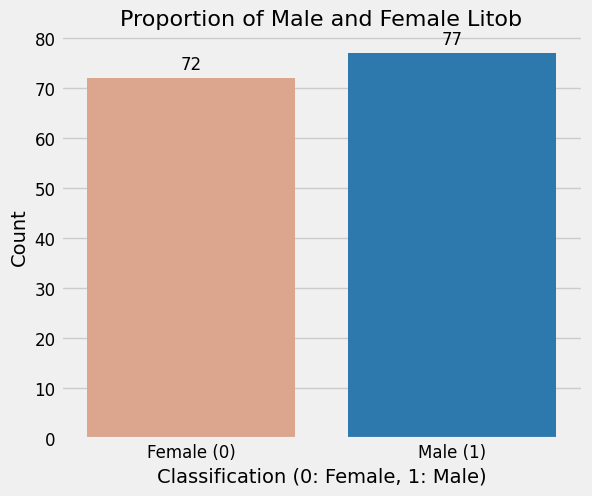
\includegraphics[width=0.6\textwidth]{figures/test-train.png}
	\caption{Proportion of Male and Female \Tgranosa}
	\label{fig:test-train}
\end{figure}

\subsection{Preprocessing Results}

\begin{table}[H]
	\centering
	{\fontsize{8}{10}\selectfont 
		\resizebox{\linewidth}{!}{ 
			\begin{tabular}{lcccc}
				\hline
				\textbf{Feature} & \textbf{$Mean \pm SD$} & \textbf{Min} & \textbf{Max} & \textbf{p-value}  \\ \hline
				Length              & $46.41 \pm 5.01$ & 38.050000 & 64.800000 & 0.036142  \\
				Width               & $35.66 \pm 3.78$ & 28.250000 & 45.500000 & 0.255091  \\
				Height              & $32.10 \pm 3.59$ & 23.350000 & 45.050000 & 0.000577  \\
				Rib count           & $19.65 \pm 0.88$ & 17.000000 & 22.000000 & 0.333161  \\
				Length (Hinge Line) & $28.06 \pm 4.24$ & 20.050000 & 43.050000 & 0.020658  \\
				Distance Umbos      & $3.25 \pm 2.85$ & 1.050000 & 35.050000 & 0.000874  \\
				LW\_ratio            & $1.30 \pm 0.07$ & 1.114710 & 1.692185 & 0.026395  \\
				LH\_ratio            & $1.45 \pm 0.10$ & 1.191919 & 1.844398 & 0.086674  \\
				\hline
			\end{tabular}
		}
	}
	\caption{ Descriptive statistics of the \Tgranosa features}
	\label{tab:descriptive-stat}
\end{table}


\section{Comparison of Model Performance}
\begin{figure}[!htbp]
	\centering
	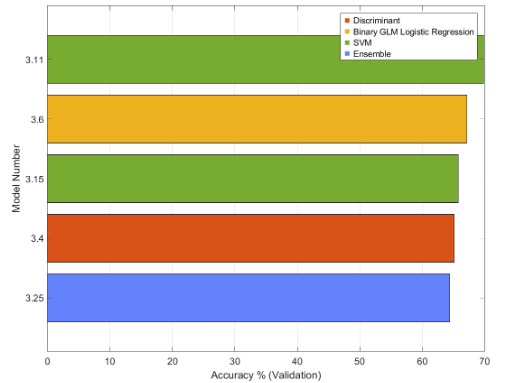
\includegraphics[width=0.6\textwidth]{figures/compare-models.png}
	\caption{Comparison of Model Performance}
	\label{fig:compare-models}
\end{figure}

Figure ~\ref{fig:compare-models} shows the comparison of the accuracy in classifying sex of \textit{T.granosa} across different models such as Discriminant, Binary GLM Logistic Regression, SVM, and Ensemble. Based on the figure ~\ref{fig:compare-models} above the SVM obtained the highest accuracy percentage. This indicates that the SVM performed best among other models in the validation set. Followed by the Binary GLM Logistic Regression then the Discriminant. On the other hand, the Ensemble has the lowest accuracy making it the worst model to perform in the validation set. 

\subsection{Performance Evaluation}

To evaluate the performance of the different models used, the effectiveness of the models was evaluated and compared in predicting the sex of the \textit{T.granosa} based on morphometric characteristics. The use of performance metrics such as accuracy, precision, recall, and F1-score are used to evaluate the performance of the different models. By analyzing the performance metrics the researchers can identify the most effective and best model for the classification of male and female \textit{T.granosa}. 


\begin{table}[H]
	\centering
	\resizebox{\linewidth}{!}{ 
		\begin{tabular}{lccccc}
			\hline
			\textbf{Model} & \textbf{Accuracy (Validation)} & \textbf{ Weighted Precision} & \textbf{ Weighted Recall} & \textbf{Weighted F1-score} & \textbf{Training Time (sec)} \\ \hline
			Linear SVM          & 69.80(\%) & 69.82(\%) & 69.80(\%) & 69.73(\%) & 2.354 \\
			Binary GLM Logistic Regression    & 67.11 (\%) & 67.16(\%) & 67.11(\%) & 66.99(\%) & 1.9415 \\
			Medium Gaussian SVM       & 65.77(\%) & 65.77(\%) & 65.77(\%) & 65.69 (\%) & 1.0323 \\
			Linear Discriminant       & 65.10(\%) & 65.22(\%) & 65.10(\%) & 64.86(\%) & 2.333\\
			Subspace Discriminant     & 64.43(\%) & 64.50(\%) & 64.43(\%) & 64.23(\%) & 7.708 \\ \hline
		\end{tabular}
	}
	\caption{Model Performance Comparison}
	\label{tab:model-performance}
\end{table}

Table ~\ref{tab:model-performance} presents the comparison results of machine learning models on the morphometric characteristics of the combined- male and female \textit{T.granosa} datasets. The results indicate that all models demonstrated moderate to high performance in predicting males and females, with accuracies ranging between 64.43\% to 69.80\%. 

The Linear SVM performs as the best model achieving the highest accuracy (69.80\%), precision (69.82\%), recall (69.80\%), and F1-score (69.73\%), with a training time of 2.354s. This indicates that SVM is well-suited in identifying sex of \textit{T.granosa} based on its morphological features. 

The Binary GLM Logistic Regression also performed well having an accuracy of (67.11\%), precision (67.16\%), recall (67.11\%), and F1-score (66.99\%), with a training time of 1.9415s which is faster than Linear SVM. 

The Medium Gaussian SVM, and Linear Discriminant closely followed each other with accuracies of (65.77\%) and (65.10\%), precisions of (65.77\%) and (65.22\%), recall of (65.77\%) and (65.10\%), and F1-score of (65.69\%) and (64.86\%), with a training time of 1.0323s and 2.333s, respectively. 

The Subspace discriminant, however, performs as the worst classifier with an accuracy of (64.43\%), precision (64.50\%), recall(64.43\%), and F1-score (64.23\%), with a having the longest training time of 7.708s. 

Overall, the results seen in this comparison highlight that machine learning models are effective in predicting sex identification of \textit{T.granosa} based on their morphometric characteristic with Linear SVM performing as the best model for this dataset. 


\subsection{Confusion Matrix Analysis}
\begin{figure}[!htbp]
	\centering
	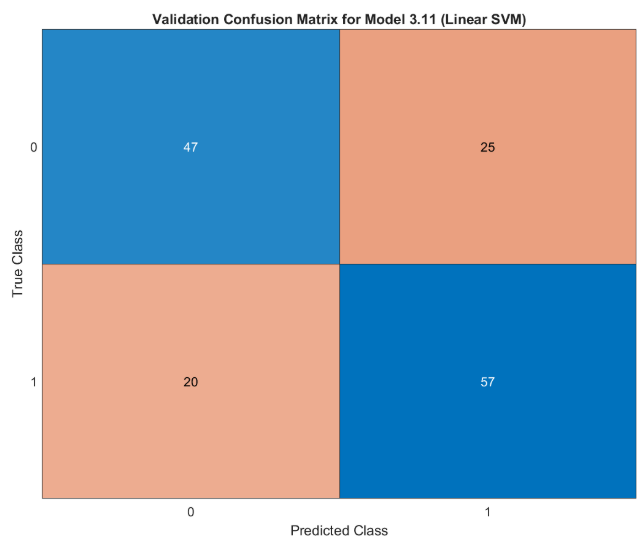
\includegraphics[width=0.6\textwidth]{figures/confusion-matrix.png}
	\caption{Confusion Matrix of Linear SVM}
	\label{fig:confusion-matrix}
\end{figure}

Figure ~\ref{fig:confusion-matrix} shows the confusion matrices that allow for a detailed breakdown of classifier predictions including true positives (correctly identified females), true negatives (correctly identified males), false positives (males incorrectly classified as females), and false negatives (females incorrectly classified as males).

Linear SVM being the best performing model had achieved 57 true positives and 47 true negatives. However, there were also 25 false positives and 20 false negatives. This indicates that the model did not accurately differentiate  between male and female, agreeing with its accuracy (69.80\%). The large number of wrongly classified data points can only indicate that while Linear SVM is the best model compared to others it still suffers from the complexity of this dataset. 

\newpage
\subsection{Feature Importance Analysis}

\begin{figure}[!htbp]
	\centering
	\begin{minipage}{0.48\textwidth} 
		\centering
		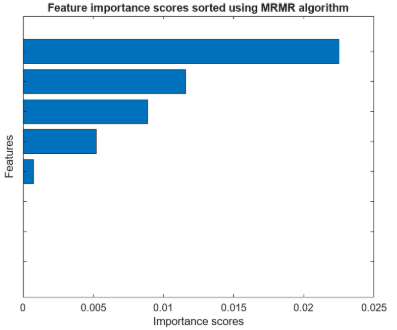
\includegraphics[width=\textwidth, height=5cm]{figures/mrmr.png} 
	\end{minipage}%
	\hfill 
	\begin{minipage}{0.48\textwidth} 
		\centering
		{\fontsize{12}{15}\selectfont 
			\begin{tabular}{p{0.5\linewidth}c}
				\hline
				\textbf{Features} & \textbf{MRMR Scores} \\ \hline
				Height              & 0.0225  \\
				Lw\_ratio           & 0.0116  \\
				DistanceUmbos       & 0.0089  \\
				RibCount            & 0.0052  \\
				Length              & 0.0007  \\
				\hline
			\end{tabular}
		}
	\end{minipage}
	\caption{Feature Importance Scores Sorted Using the MRMR Algorithm.}
	\label{fig:mrmr-combined}
\end{figure}

\begin{figure}[!htbp]
	\centering
	\begin{minipage}{0.48\textwidth} 
		\centering
		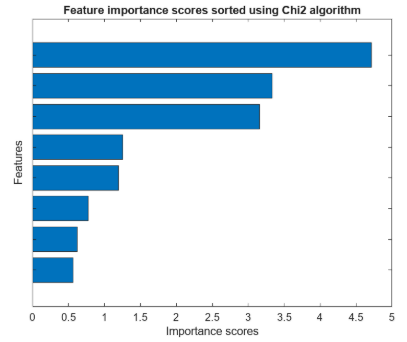
\includegraphics[width=\textwidth, height=5cm]{figures/chi2.png} 
	\end{minipage}%
	\hfill 
	\begin{minipage}{0.48\textwidth} 
		\centering
		{\fontsize{12}{15}\selectfont 
			\begin{tabular}{p{0.5\linewidth}c}
				\hline
				\textbf{Features} & \textbf{Chi2 Scores}   \\ \hline
				DistanceUmbos       & 4.7164   \\
				Height              & 3.3334  \\
				Length\_Hinge\_Line & 3.1542  \\
				LW\_ratio           & 1.2570  \\
				Length              & 1.1934  \\
				RibCount            & 0.7718 \\
				LH\_ratio           & 0.6241 \\ 
				Width               & 0.5611 \\ 
				\hline
			\end{tabular}
		}
	\end{minipage}
	\caption{Feature Importance Scores Sorted Using the Chi2 Algorithm.}
	\label{fig:chi2-combined}
\end{figure}

\begin{figure}[!htbp]
	\centering
	\begin{minipage}{0.48\textwidth} 
		\centering
		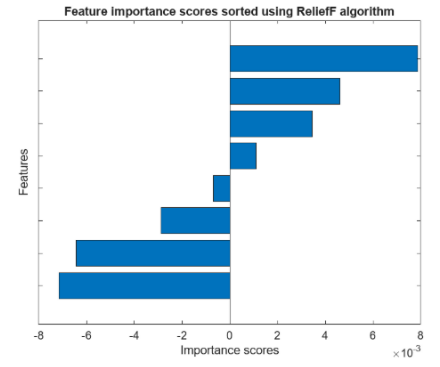
\includegraphics[width=\textwidth, height=5cm]{figures/reliefF.png} 
	\end{minipage}%
	\hfill 
	\begin{minipage}{0.48\textwidth} 
		\centering
		{\fontsize{12}{15}\selectfont 
			\begin{tabular}{p{0.5\linewidth}c}
				\hline
				\textbf{Features} & \textbf{ReliefF Scores}   \\ \hline
				DistanceUmbos       & 0.0079   \\
				Length              & 0.0046  \\
				Width               & 0.0034  \\
				Length\_Hinge\_Line & 0.0011  \\
				\hline
			\end{tabular}
		}
	\end{minipage}
	\caption{Feature Importance Scores Sorted Using the ReliefF Algorithm.}
	\label{fig:reliefF-combined}
\end{figure}

\begin{figure}[!htbp]
	\centering
	\begin{minipage}{0.48\textwidth} 
		\centering
		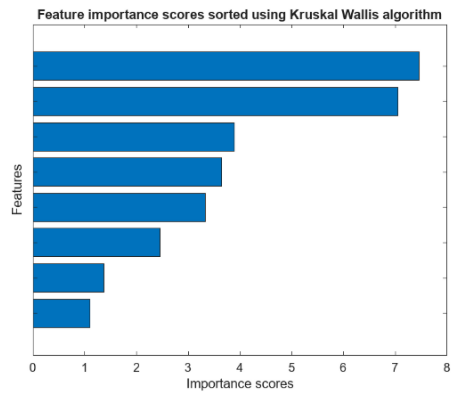
\includegraphics[width=\textwidth, height=5cm]{figures/kw.png} 
	\end{minipage}%
	\hfill 
	\begin{minipage}{0.48\textwidth} 
		\centering
		{\fontsize{10}{12}\selectfont 
			\begin{tabular}{p{0.5\linewidth}c}
				\hline
				\textbf{Features} & \textbf{Kruskal Wallis Scores}   \\ \hline
				Height              & 7.4640  \\
				DistanceUmbos       & 7.0491  \\
				Length\_Hinge\_Line & 3.8847  \\
				LW\_ratio           & 3.6395  \\
				Length              & 3.3250 \\ 
				LH\_ratio           & 2.4496 \\
				Width               & 1.3692 \\
				RibCount            & 1.1022 \\
				\hline
			\end{tabular}
		}
	\end{minipage}
	\caption{Feature Importance Scores Sorted Using the Kruskal Wallis Algorithm.}
	\label{fig:kw-combined}
\end{figure}


After processing the dataset and splitting it into training and testing sets, the models are trained and their important features are computed. Feature Analysis helps in identifying which morphological features contribute most in classifying male and female \textit{T.granosa}. The study uses models such as Minimum Redundancy Maximum Relevance (mRMR), Chi-square (Chi2), ReliefF, Analysis of Variance (ANOVA) and Kruskal Wallis feature selection algorithms. 

The Minimum Redundancy Maximum Relevance (mRMR) has the best features of height, LW ratio, distance of the umbos, rib count, and length respectively that contribute most in identifying sex classification. The Chi-square (Chi2) includes all 8 features however, the distance of the umbos contributes the most followed by height, length of the hinge, LW ratio, length, rib count, LH ratio and width. In the ReliefF scores its best features include the distance of the umbos, length, width, and length of the hinge however, height, LW ratio, LH ratio, and rib count did not contribute in the sex classification. Moreover, in Kruskal Wallis the height contributes the most followed by the distance of the umbos, length of the hinge, LW ratio, length, LH ratio, width, and rib count as the lowest. 

The results in figures ~\ref{fig:mrmr-combined},  ~\ref{fig:chi2-combined},  ~\ref{fig:reliefF-combined}, and ~\ref{fig:kw-combined} indicates variations in feature importance between the four algorithm models, however certain features such as the distance of the umbos are present in all algorithm best features, and followed along the height that are the best features of the three algorithms except for ReliefF. Therefore, features such as distance of the umbos and height consistently emerge as influential predictors. Hence, this analysis allowed the researchers to identify which features were most predictive and can serve as a baseline for sex identification of \textit{T.granosa} based on morphological features. 




